\documentclass[journal]{IEEEtran}
\usepackage[T1]{fontenc}
\usepackage{lmodern}
\usepackage[spanish]{babel}
\usepackage[utf8]{inputenc}
\usepackage{amsmath}
\usepackage{graphicx}
\graphicspath{{figuras/}}
 
\begin{document}
 
\title{Escuchar y ver: diseño e implementación de un sistema de ambientación visual reactiva para audiolibros}
\author{Bernardita Robles}
 
\maketitle
 
\begin{abstract}
% MÓDULO 4
\end{abstract}
 
% =====================================================================
\section{Introducción}
% MÓDULO 4 - Se redacta al final. Por ahora contiene problemática,
% objetivo e investigación bibliográfica (consigna del Módulo 3).
 
\subsection{Problemática}
% PENDIENTE: agregar una cita con un dato sobre el crecimiento del consumo de audiolibros.
El consumo de audiolibros ha crecido fuertemente, pero la experiencia sigue siendo puramente auditiva. Al escuchar una narración, el oyente construye imágenes mentales propias, y la combinación de información verbal y no verbal puede favorecer el recuerdo \cite{paivio1991}. Sin embargo, no se sabe si un estímulo visual generado automáticamente potencia esa experiencia o interfiere con la imaginación de quien escucha. Hasta donde se pudo relevar, las aplicaciones actuales reproducen audiolibros, pero no acompañan la escucha de un libro completo con una ambientación visual dinámica.
 
\subsection{Objetivo general}
Diseñar e implementar una prueba de concepto de un sistema que genera una ambientación visual reactiva sincronizada con la narración de un audiolibro, cuyas reglas de diseño se derivan de la Teoría de la Codificación Dual, la Teoría Cognitiva del Aprendizaje Multimedia y el concepto de \textit{ambient display}, y proponer un diseño experimental para evaluar su efecto sobre la comprensión, la inmersión y la fatiga visual del oyente en comparación con la escucha sin estímulo visual.
 
\subsection{Investigación bibliográfica}
% Temporal: en el Módulo 4 esta lista desaparece y las referencias
% se integran en la introducción.
 
\begin{enumerate}
 
\item \textbf{Paivio (1991)} \cite{paivio1991}. Revisión de la Teoría de la Codificación Dual: un sistema verbal y otro no verbal, conectados entre sí.
 
\item \textbf{Paivio (1986)} \cite{paivio1986}. Desarrollo completo del modelo (\textit{logogens} e \textit{imagens}) y de las conexiones referenciales.
 
\item \textbf{Mayer (2009)} \cite{mayer2009}. Teoría Cognitiva del Aprendizaje Multimedia (CTML) y sus principios de diseño.
 
\item \textbf{Mayer y Moreno (2003)} \cite{mayermoreno2003}. Escenarios de sobrecarga cognitiva y estrategias para reducirla.
 
\item \textbf{Mayer (2024)} \cite{mayer2024}. Revisión actualizada de la CTML y de sus herramientas de medición.
 
\item \textbf{Rogowsky et al. (2016)} \cite{rogowsky2016}. Comprensión en lectura, escucha y modalidad dual.
 
\item \textbf{Mousavi et al. (1995)} \cite{mousavi1995}. Reducción de la carga cognitiva al distribuir información entre canal auditivo y visual.
 
\item \textbf{Green y Brock (2000)} \cite{greenbrock2000}. Concepto de transporte narrativo y escala para medirlo.
 
\item \textbf{Green y Brock (2002)} \cite{greenbrock2002}. Modelo de transporte e imaginería.
 
\item \textbf{Wisneski et al. (1998)} \cite{wisneski1998}. Concepto de \textit{ambient display}.
 
\item \textbf{Xie et al. (2023)} \cite{xie2023}. Seguimiento cortical del habla bajo atención dividida entre audio y una tarea visual.
 
\item \textbf{Wilms y Oberfeld (2018)} \cite{wilmsoberfeld2018}. Efecto del matiz, la saturación y el brillo sobre la emoción.
 
\item \textbf{Graf et al. (2021)} \cite{graf2021}. Sistema de visualización musical en tiempo real a partir de rasgos del audio.
 
\item \textbf{Radford et al. (2023)} \cite{radford2023}. Whisper: reconocimiento de habla con marcas temporales, usado para sincronizar texto y audio en el sistema.
 
\item \textbf{Russell (1980)} \cite{russell1980}. Modelo circumplejo del afecto (valencia y activación), usado para anotar el tono emocional de cada segmento.
 
\item \textbf{Appel et al. (2015)} \cite{appel2015}. Versión breve de la escala de transporte narrativo, propuesta como medida de inmersión.
 
\item \textbf{Seguí et al. (2015)} \cite{segui2015}. Cuestionario validado de síntomas visuales asociados al uso de pantallas, propuesto como medida de fatiga visual.
 
\item \textbf{Lakens (2017)} \cite{lakens2017}. Guía práctica de pruebas de equivalencia, propuesta para evaluar si la ambientación mínima no empeora la comprensión.
 
\end{enumerate}
 
% =====================================================================
\section{Antecedentes}
 
\subsection{Modalidad de presentación y comprensión}
La evidencia sobre el efecto del formato en la comprensión de un texto es inconsistente. Rogowsky et al. \cite{rogowsky2016} dividen a un conjunto de universitarios con inglés como lengua nativa en tres grupos: lectura, escucha de un audiolibro y modalidad dual (ambas a la vez). Con un mismo capítulo de no ficción narrativa, no hallan diferencias significativas de comprensión ni en una evaluación inmediata ni en otra a las dos semanas. Los autores atribuyen la discrepancia con estudios que favorecen la lectura (Daniel y Woody, 2010, citado en \cite{rogowsky2016}) a que allí los participantes podían repasar el material, y la discrepancia con estudios sobre modalidad dual (Chang, 2009; Diao y Sweller, 2007, citados en \cite{rogowsky2016}) a que estos trabajan con estudiantes de inglés como segunda lengua.
 
Por lo tanto, el efecto de la modalidad parece depender de la tarea y del perfil de los participantes, sumado a que los resultados provienen de un único texto de no ficción.
 
\subsection{Atención dividida entre audio y estímulo visual}
Xie et al. \cite{xie2023} evalúan a 16 adultos jóvenes que escuchan fragmentos de alrededor de un minuto de \textit{Alicia en el país de las maravillas} en tres condiciones: solo escucha, escucha con una tarea visual de baja carga y escucha con una tarea visual de alta carga. La precisión en las preguntas de comprensión es de 89\,\%, 85\,\% y 66\,\%, respectivamente; solo la condición de alta carga difiere significativamente de la escucha sin tarea.
 
Mayer y Moreno \cite{mayermoreno2003} explican este tipo de efectos por la capacidad limitada de procesamiento: los elementos de la presentación que no son necesarios para comprender el contenido generan un procesamiento incidental, que consume parte de la capacidad limitada del oyente y reduce la disponible para procesar el contenido esencial. En cinco estudios, agregar música de fondo o videos irrelevantes a animaciones narradas reduce el aprendizaje. Los autores aclaran, además, que un material puede estar relacionado con el tema y aun así resultar ajeno si no contribuye al objetivo.
 
\subsection{Visualización reactiva y estímulos ambientales}
Graf et al. \cite{graf2021} desarrollan un sistema que transforma rasgos de una señal de audio, como el volumen y los cambios de intensidad, en parámetros de una escena visual en tiempo real. En su evaluación, 34 participantes califican de 1 a 10 el ajuste entre música e imagen; las dos visualizaciones reactivas obtienen 7,1 y 6,8, frente a 4,5 de una visualización no reactiva. El estudio usa una sola canción de un minuto y no mide comprensión ni inmersión.
 
Wisneski et al. \cite{wisneski1998} proponen los \textit{ambient displays}: interfaces que comunican información mediante cambios sutiles de luz, sonido y movimiento, y son procesables en el trasfondo, por lo que requieren menor atención. Por otra parte, Wilms y Oberfeld \cite{wilmsoberfeld2018} muestran a 62 participantes colores que varían en matiz, saturación (intensidad del color) y brillo, y les piden calificar su activación (cuánta alerta les generan) y su valencia (cuán agradables les resultan). Los colores más saturados y brillantes generan mayor activación, y el matiz influye solo en saturaciones medias y altas. En cambio, ningún color se percibe como claramente agradable o desagradable. Dado que los colores se presentan de forma estática en una cabina oscura, no está establecido que estos resultados se mantengan en otros contextos.
 
Ninguno de estos trabajos implementa ni evalúa una ambientación visual reactiva durante la escucha de un audiolibro de ficción completo.
 
% =====================================================================
\section{Marco teórico}
 
\subsection{Teoría de la Codificación Dual}
La Teoría de la Codificación Dual \cite{paivio1986, paivio1991} sostiene que la mente procesa la información mediante un sistema verbal y uno no verbal, con unidades propias (\textit{logogens} e \textit{imagens}) vinculadas por conexiones referenciales. Representar una misma información en ambos sistemas favorece su recuerdo. En un audiolibro, la narración activa el sistema verbal y las imágenes que construye el oyente activan el no verbal. Una ambientación visual externa puede sumarse a esas imágenes o competir con ellas; la teoría no determina cuál de los dos efectos predomina, y la propia revisión de Paivio \cite{paivio1991} discute objeciones a que los códigos se sumen de forma independiente.
 
\subsection{Teoría Cognitiva del Aprendizaje Multimedia}
La CTML \cite{mayer2009, mayer2024} supone dos canales de procesamiento (auditivo-verbal y visual-pictórico), cada uno de capacidad limitada, y un procesamiento activo de selección, organización e integración. Distingue procesamiento esencial, extraño (incidental en \cite{mayermoreno2003}) y generativo; el extraño consume capacidad sin contribuir al objetivo. De allí se derivan dos principios relevantes: el de coherencia, que recomienda eliminar material atractivo pero ajeno, y el de modalidad, según el cual presentar palabras como narración y no como texto en pantalla libera el canal visual \cite{mayermoreno2003, mousavi1995}. La CTML se desarrolla con material académico y pruebas de transferencia, por lo que en este trabajo sus principios se usan como guía para el diseño y no como predicciones directas.
 
\subsection{Transporte narrativo}
El transporte narrativo es el estado de absorción en un relato, en el que la atención, la imaginería y las emociones se concentran en la historia \cite{greenbrock2000}. Su intensidad depende de la capacidad del relato para evocar imágenes mentales vívidas \cite{greenbrock2002}. El transporte se mide mediante una escala autoadministrada \cite{greenbrock2000}, con una versión breve validada \cite{appel2015}. En este trabajo, el transporte se usa para medir la inmersión. Además, como depende de las imágenes que construye el propio oyente, el estímulo visual evita mostrar figuras.
 
% =====================================================================
\section{Diseño del sistema}
 
\subsection{Requisitos derivados}
A partir de los antecedentes y del marco teórico se definen cinco requisitos para el estímulo visual:
 
\begin{itemize}
\item \textbf{R1 -- Sin interacción.} El estímulo no exige respuestas ni seguimiento activo, a diferencia de las tareas visuales que reducen la comprensión \cite{xie2023}.
\item \textbf{R2 -- Cambios lentos y sutiles.} Las transiciones de color y el movimiento del estímulo son lentos, para que se procesen en el trasfondo de la atención \cite{wisneski1998}.
\item \textbf{R3 -- No figurativo.} El estímulo se limita a color, luz difusa y una textura abstracta en movimiento, sin objetos ni escenas que reemplacen la imaginería del oyente \cite{greenbrock2002}.
\item \textbf{R4 -- Coherente con la narración.} Los cambios responden al contenido de la historia, para no constituir material ajeno según el principio de coherencia \cite{mayermoreno2003}.
\item \textbf{R5 -- Saturación y brillo moderados.} Valores moderados limitan el aumento de la activación \cite{wilmsoberfeld2018}.
\end{itemize}
 
\subsection{Arquitectura}
El sistema se divide en dos etapas que operan en momentos distintos. La primera es la etapa de preprocesamiento, que se ejecuta una sola vez por audiolibro y produce un archivo con la anotación afectiva de la narración. La segunda etapa es la de reproducción, que se ejecuta durante la escucha y genera la ambientación en tiempo real a partir de ese archivo. Se separa en dos etapas porque cada una tiene tiempos muy distintos: la transcripción y el análisis del texto requieren varios minutos de cómputo, mientras que la reproducción debe actualizar la imagen decenas de veces por segundo. Además, un mismo archivo de anotación sirve para todas las condiciones experimentales, que difieren solo en los parámetros del reproductor.
 
\subsubsection{Preprocesamiento}
 
La etapa de preprocesamiento consta de tres módulos encadenados.
 
\textbf{Transcripción y sincronización.} La entrada es el archivo de audio de la narración. Whisper \cite{radford2023} lo transcribe y devuelve, para cada frase, su texto y sus tiempos de inicio y fin. Gracias a estos tiempos, el sistema sabe qué se está narrando en cada momento, de modo que la ambientación corresponde a esa parte de la historia.
 
\textbf{Segmentación.} Las frases consecutivas se agrupan en segmentos de una duración mínima $d_{\min} = 20$~s: un segmento se cierra en el primer final de frase posterior a ese umbral. De este modo, cada segmento conserva oraciones completas y el valor objetivo del estímulo cambia, como máximo, una vez cada 20~s (R2). Un umbral menor produciría cambios frecuentes, y uno mayor omitiría cambios de tono dentro de la narración.
 
\textbf{Anotación afectiva.} Un modelo de lenguaje recibe el texto de cada segmento junto con el del segmento anterior, para que la valoración considere el contexto de la escena. Para cada segmento $i$ devuelve una valencia $v_i \in [-1, 1]$, que indica cuán agradable o desagradable es el contenido, y una activación $a_i \in [0, 1]$, que indica su intensidad, siguiendo las dos dimensiones del modelo circumplejo del afecto \cite{russell1980}. La instrucción define ambas dimensiones y exige una respuesta en formato JSON, lo que permite procesarla de forma automática. La anotación se realiza sobre el texto y no sobre el audio, porque el estímulo debe reflejar el contenido de la historia para no constituir material ajeno (R4).
 
El resultado del preprocesamiento es un archivo JSON con un registro por segmento, que contiene sus tiempos de inicio y fin, su texto, las frases que lo componen con sus tiempos y sus valores afectivos.
 
\subsubsection{Reproducción}
El reproductor es una página web que reproduce el audio y muestra la ambientación a pantalla completa. En cada cuadro de animación, aproximadamente 60 veces por segundo, ejecuta cuatro pasos:
 
\begin{enumerate}
\item \textbf{Lectura del audio.} Obtiene la posición de reproducción $t$ y la energía de la señal en ese instante, normalizada como $r(t) \in [0, 1]$.
\item \textbf{Búsqueda del segmento activo.} Identifica en el archivo JSON el segmento $i$ cuyo intervalo contiene a $t$.
\item \textbf{Cálculo del color y del movimiento.} Obtiene los valores objetivo de matiz, saturación y luminosidad a partir de $a_i$ y $v_i$, los aproxima de forma gradual y suma una leve modulación según la intensidad de la voz, siguiendo el enfoque de Graf et al. \cite{graf2021}. A partir de la activación, también calcula la velocidad y la turbulencia de la textura.
\item \textbf{Renderizado.} Dibuja a pantalla completa un campo de niebla abstracta en movimiento, cuyo color medio es el calculado en el paso anterior, sin formas ni figuras (R3).
\end{enumerate}
 
El reproductor no ofrece más controles que los de reproducción, por lo que el oyente no necesita interactuar con el estímulo (R1). Los parámetros del mapeo se agrupan en perfiles, que se seleccionan al iniciar la sesión.
 
\subsection{Mapeo de la narración al estímulo}
El color se representa en el espacio HSL (matiz $H$, saturación $S$ y luminosidad $L$). Para cada segmento $i$ se calculan los valores objetivo:
\begin{align}
S_i^{*} &= S_{\min} + a_i\,(S_{\max} - S_{\min}) \label{eq:s}\\
L_i^{*} &= L_{\min} + a_i\,(L_{\max} - L_{\min}) \label{eq:l}\\
H_i^{*} &= H_0 + v_i\,\Delta H \label{eq:h}
\end{align}
donde $a_i$ y $v_i$ son la activación y la valencia del segmento, $[S_{\min}, S_{\max}]$ y $[L_{\min}, L_{\max}]$ son los rangos permitidos de saturación y luminosidad, $H_0$ es el matiz base de la obra y $\Delta H$ es el desplazamiento máximo de matiz. La activación controla saturación y luminosidad porque son las dimensiones con mayor efecto sobre la activación emocional \cite{wilmsoberfeld2018}. La valencia solo desplaza el matiz dentro de un rango acotado, ya que su relación con el color es débil \cite{wilmsoberfeld2018}.
 
Para cumplir R2, cada parámetro $p \in \{H, S, L\}$ se aproxima a su valor objetivo $p^{*}$ mediante un suavizado exponencial:
\begin{equation}
p(t + \Delta t) = p(t) + \left(1 - e^{-\Delta t/\tau}\right)\left(p^{*} - p(t)\right)
\label{eq:suavizado}
\end{equation}
donde $\Delta t$ es el intervalo entre cuadros y $\tau$ es la constante de tiempo de la transición. Finalmente, la luminosidad mostrada incorpora la intensidad de la voz:
\begin{equation}
L(t) = L_{s}(t) + k\, r(t)
\label{eq:intensidad}
\end{equation}
donde $L_{s}(t)$ es la luminosidad suavizada, $r(t) \in [0, 1]$ es la energía RMS normalizada de la señal de audio y $k$ es la ganancia de modulación.

El color $(H, S, L)$ obtenido es el valor medio del estímulo. Sobre él se dibuja una textura de ruido fractal, que varía la luminosidad en una proporción $c$ (contraste) y el matiz en hasta $\pm\delta_H$ grados alrededor de ese valor, y que se desplaza de forma continua. La activación también controla el movimiento: a partir de la activación suavizada $a_s(t)$, obtenida con la misma ecuación~\eqref{eq:suavizado}, se calculan la velocidad de deriva $u$ y la turbulencia $w$ de la textura:
\begin{align}
u(t) &= u_{\min} + a_s(t)\,(u_{\max} - u_{\min}) \label{eq:vel}\\
w(t) &= w_{\min} + a_s(t)\,(w_{\max} - w_{\min}) \label{eq:turb}
\end{align}
La velocidad se integra en una fase, $\varphi(t + \Delta t) = \varphi(t) + u(t)\,\Delta t$, que desplaza la textura. Así, un cambio de activación modifica el ritmo del movimiento sin producir saltos en la imagen. Las escenas calmas se ven casi quietas, y las intensas, más rápidas y turbulentas.
 
Todos los parámetros se agrupan en perfiles configurables. El perfil \textit{mínimo} cumple los cinco requisitos; el perfil \textit{llamativo} no cumple R2 ni R5, ya que usa cambios y movimientos rápidos y colores intensos, y se usa como condición de contraste en la evaluación (Tabla~\ref{tab:perfiles}). La velocidad $u$ se expresa en unidades de textura por segundo: con $u = 0{,}02$, una forma de la niebla tarda alrededor de 50~s en recorrer su propio tamaño.
 
\begin{table}[t]
\centering
\caption{Perfiles de ambientación}
\label{tab:perfiles}
\begin{tabular}{lcc}
\hline
Parámetro & Mínimo & Llamativo \\
\hline
$[S_{\min}, S_{\max}]$ & $[0{,}20;\ 0{,}45]$ & $[0{,}70;\ 1{,}00]$ \\
$[L_{\min}, L_{\max}]$ & $[0{,}15;\ 0{,}35]$ & $[0{,}40;\ 0{,}65]$ \\
$\Delta H$ & $20^\circ$ & $60^\circ$ \\
$\tau$ & 6~s & 0,5~s \\
$k$ & 0,02 & 0,15 \\
$[u_{\min}, u_{\max}]$ & $[0{,}012;\ 0{,}05]$ & $[0{,}10;\ 0{,}60]$ \\
$[w_{\min}, w_{\max}]$ & $[0{,}25;\ 0{,}65]$ & $[0{,}60;\ 1{,}40]$ \\
$c$ & 0,30 & 0,60 \\
$\delta_H$ & $8^\circ$ & $35^\circ$ \\
\hline
\end{tabular}
\end{table}
 
% =====================================================================
\section{Implementación de la prueba de concepto}

\subsection{Preprocesamiento}
El preprocesamiento se implementa en Python. La transcripción usa el modelo \textit{small} de Whisper \cite{radford2023}, que devuelve el texto de cada frase con sus marcas temporales. La segmentación agrupa las frases según la regla de $d_{\min} = 20$~s descrita en la Sección~IV.

El módulo de anotación afectiva envía cada segmento, junto con el anterior, a la API de un modelo de lenguaje con una instrucción que define la valencia y la activación y exige una respuesta en JSON. Antes de escribir cada respuesta en el archivo de salida, verifica que tenga el formato y los rangos esperados; si no los cumple, el segmento se vuelve a anotar. En la prueba de concepto no se contó con acceso a la API, por lo que la anotación de la obra la realizó el modelo Claude (Anthropic) en una sesión interactiva, siguiendo la misma instrucción y el mismo esquema: cada segmento se valoró leyendo también el anterior, y los valores pasaron por la misma validación de formato y rangos. Por eso, esta anotación no puede reproducirse ejecutando el módulo, aunque los valores y la instrucción quedan registrados.

\subsection{Reproductor}
El reproductor se implementa en JavaScript como una página web autocontenida, sin dependencias externas. El audio se reproduce con el elemento \texttt{audio} de HTML5, y la Web Audio API, mediante un \texttt{AnalyserNode}, entrega la señal para calcular $r(t)$. Para que $r(t)$ no dependa del volumen de la grabación, la energía RMS se divide por un máximo que decae lentamente, con una constante de 30~s. El ciclo de animación se sincroniza con la frecuencia de actualización de la pantalla mediante \texttt{requestAnimationFrame}. Como los segmentos están ordenados en el tiempo, el segmento activo se localiza mediante búsqueda binaria, y en los huecos entre segmentos se mantiene el último segmento iniciado.

La niebla se dibuja con WebGL sobre un elemento \texttt{canvas}, mediante un programa de sombreado que combina varias capas de ruido fractal deformadas entre sí, a una resolución reducida, ya que la imagen es difusa. Si el navegador no dispone de WebGL, el reproductor dibuja en su lugar un gradiente radial difuso con el mismo color. En la condición de control, la pantalla muestra un gris neutro y estático ($L = 0{,}25$).

El reproductor tiene dos modos. En el modo \textit{experimento}, la ambientación ocupa toda la pantalla, sin cursor ni controles; los intentos de pausar o de saltar en el audio se bloquean y quedan registrados. Al terminar, la sesión genera un registro con cada cambio de segmento, su desfase y la tasa de cuadros de cada segundo. En el modo \textit{desarrollo}, se agrega un panel que muestra la frase que se está narrando, una línea de tiempo de la obra con la valencia, la activación y el color objetivo de cada segmento, y los valores actuales del estímulo. Este panel sirve para inspeccionar y demostrar el sistema, y no se muestra a los participantes.

\subsection{Obra}
La prueba de concepto se aplica a \textit{La mujer alta}, cuento de Pedro Antonio de Alarcón escrito originalmente en español, en una grabación de dominio público de LibriVox con un único narrador, de 36~min 16~s de duración. Se eligió por ser una historia completa de una duración apta para una sesión experimental y con un arco emocional variado: comienza con una conversación distendida entre amigos y avanza hacia escenas de duelo y de terror, con regresos a la conversación inicial.

Whisper transcribió el audio en unos seis minutos, en un equipo de cuatro núcleos sin GPU, y produjo 612 frases. La segmentación las agrupó en 100 segmentos, de entre 20 y 27~s (21,7~s en promedio). La Fig.~\ref{fig:anotacion} muestra la anotación resultante. La valencia media es $-0{,}48$ (87 de los 100 segmentos son negativos), y la activación media es $0{,}53$, con picos en los encuentros con la mujer alta y valores bajos en la conversación inicial y en los regresos al marco del relato.

\begin{figure}[t]
\centering
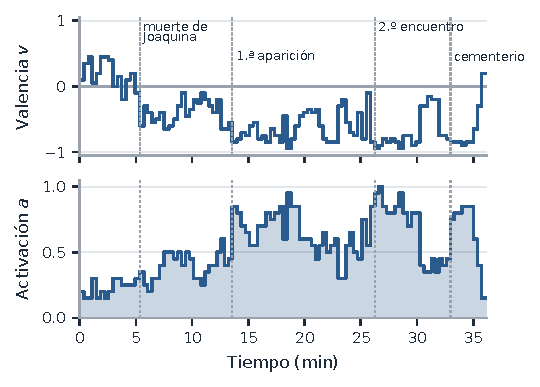
\includegraphics[width=\columnwidth]{anotacion}
\caption{Valencia y activación asignadas a cada uno de los 100 segmentos de \textit{La mujer alta}. Las líneas punteadas marcan momentos del relato.}
\label{fig:anotacion}
\end{figure}

La Fig.~\ref{fig:estimulo} muestra el estímulo de ambos perfiles en un momento de calma y en uno de terror. En el perfil mínimo, el cambio es apenas perceptible, como exige R2. En la prueba se usa un matiz base $H_0 = 210^\circ$ (azul).

\begin{figure}[t]
\centering
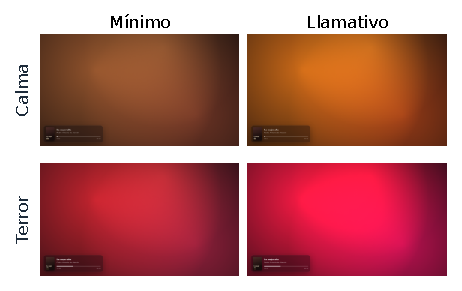
\includegraphics[width=\columnwidth]{estimulo}
\caption{Estímulo en un segmento de calma ($v = 0{,}45$, $a = 0{,}15$) y en uno de terror ($v = -0{,}85$, $a = 0{,}85$), con los perfiles mínimo y llamativo.}
\label{fig:estimulo}
\end{figure}

\subsection{Verificación técnica}
La verificación técnica evalúa tres aspectos. Primero, la sincronización: se mide el desfase entre el inicio de cada segmento y el cuadro en que el reproductor cambia de color objetivo. Segundo, la fluidez: se registra la tasa de cuadros por segundo durante una sesión completa, para comprobar que la animación no se degrada con el tiempo. Tercero, la validez de la anotación: se comparan la valencia y la activación asignadas por el modelo con las asignadas por anotadores humanos en una muestra de segmentos.

Para los dos primeros aspectos, se reprodujo la obra completa con el perfil mínimo en modo experimento, en el navegador Chromium sin interfaz gráfica y con renderizado por software, en el mismo equipo de cuatro núcleos. Los resultados se muestran en la Fig.~\ref{fig:verificacion}. En los 100 cambios de segmento, el desfase medio fue de 9,8~ms, con una mediana de 9,8~ms y un máximo de 20,2~ms; es decir, el color objetivo cambió como máximo un cuadro después del inicio de cada segmento, más el retardo con que se actualiza la posición del audio. Este desfase es despreciable frente a la constante de tiempo de la transición del perfil mínimo ($\tau = 6$~s). En cuanto a la fluidez, durante los 2157 segundos registrados la tasa media fue de 59,99 cuadros por segundo, con un mínimo de 58,0, y no se observó degradación con el tiempo: la media fue de 59,99 en el primer 10\,\% de la sesión y de 60,0 en el último. El intento de pausa realizado durante la prueba fue bloqueado y registrado, y el audio continuó hasta el final.

\begin{figure}[t]
\centering
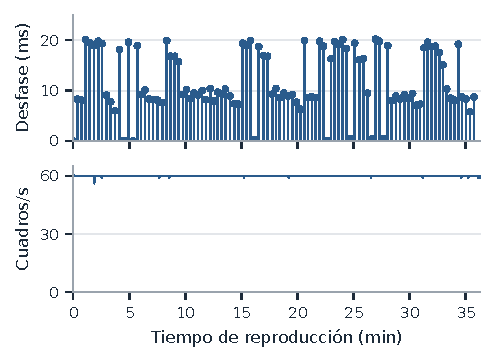
\includegraphics[width=\columnwidth]{verificacion}
\caption{Verificación técnica durante la reproducción completa con el perfil mínimo: desfase de cada cambio de segmento y cuadros por segundo.}
\label{fig:verificacion}
\end{figure}

El desfase se mide con la posición que informa el elemento \texttt{audio} en el cuadro del cambio, por lo que no incluye la latencia de salida del sonido ni la de la pantalla. Además, como la medición se hizo sin una pantalla física y con renderizado por software, debe repetirse en el equipo del experimento.

La validez de la anotación no se evaluó en este trabajo, porque no se contó con anotadores humanos en el plazo disponible. El sistema incluye las herramientas para hacerlo: una planilla con una muestra aleatoria de segmentos, sin los valores del modelo, y un análisis que calcula las correlaciones de Pearson y de Spearman y el error absoluto medio entre el modelo y el promedio humano, junto con el acuerdo entre los anotadores como referencia.

% =====================================================================
\section{Diseño experimental propuesto}
 
\subsection{Participantes y condiciones}
Se propone un diseño entre sujetos con tres condiciones: el grupo de control escucha el audiolibro con la pantalla fija, sin cambios; el segundo grupo lo escucha con una ambientación suave (perfil mínimo), y el tercero, con una ambientación exagerada (perfil llamativo). Cada participante pasa por una sola condición, lo que evita que una afecte a las siguientes y permite usar el mismo texto en los tres grupos. Los participantes son adultos con español como lengua materna, visión normal o corregida y sin conocimiento previo de \textit{La mujer alta}.
 
\subsection{Procedimiento}
Cada participante escucha la obra completa (36 minutos) frente a una pantalla, en un ambiente de iluminación controlada. Se usa una historia completa para que ningún participante escuche un relato sin final, lo que podría afectar la inmersión. En la condición de control, la pantalla muestra un fondo neutro y estático. No se permite pausar ni retroceder el audio; el reproductor lo impide en el modo experimento y registra los intentos. Antes de comenzar, el participante completa el cuestionario de fatiga visual. Al finalizar, completa las medidas de comprensión e inmersión y repite el cuestionario de fatiga visual.
 
\subsection{Medidas}
\begin{itemize}
\item \textbf{Comprensión.} Test de opción múltiple sobre hechos, personajes y secuencia de la historia.
\item \textbf{Inmersión.} Versión breve de la escala de transporte narrativo \cite{appel2015}, adaptada al español.
\item \textbf{Fatiga visual.} Cuestionario de síntomas visuales asociados a pantallas \cite{segui2015}.
\end{itemize}
 
\subsection{Análisis estadístico}
Para cada medida, las diferencias entre los tres grupos se analizan con un ANOVA de un factor y, si resultan significativas, se identifican los grupos que difieren mediante comparaciones de a pares. Sin embargo, la hipótesis de comprensión plantea que el perfil mínimo no la empeora, y la ausencia de una diferencia significativa no demuestra que dos grupos sean iguales. Por eso, la comparación entre el control y el perfil mínimo se evalúa además con una prueba de equivalencia (TOST) \cite{lakens2017}, que verifica si la diferencia entre ambos grupos es menor que un margen fijado antes de recolectar los datos. En el caso de la fatiga visual, se analiza el aumento de síntomas, calculado como la diferencia entre la medición posterior y la anterior a la sesión.
 
% =====================================================================
\section{Resultados esperados}
 
\subsection{Comprensión}
Se espera que el grupo con ambientación mínima comprenda la historia tan bien como el grupo que escucha sin estímulo visual, y que el grupo con ambientación llamativa la comprenda peor que ambos.
 
Esta expectativa se basa en que una tarea visual sencilla no afecta de forma significativa la comprensión de un audiolibro, mientras que una tarea exigente sí la reduce \cite{xie2023}. La ambientación mínima exige aún menos que una tarea sencilla, porque el oyente no tiene que hacer nada con ella. La ambientación llamativa, en cambio, al cambiar y moverse con mayor rapidez y utilizar colores más intensos, tiende a captar la atención y empeorar la comprensión de la historia \cite{mayermoreno2003}.
 
Si el grupo con ambientación mínima comprende peor que el de control, significa que el oyente percibe la ambientación como algo ajeno a la historia, aunque esté vinculada a ella, y el sistema necesitaría cambios todavía más suaves.
 
\subsection{Inmersión}
Se espera que la ambientación mínima mantenga o aumente la inmersión en la historia, y que la llamativa la reduzca.
 
La inmersión depende de que el oyente concentre su atención en la historia, imagine las escenas y se involucre emocionalmente \cite{greenbrock2000}. La ambientación mínima no muestra figuras, por lo que deja intactas las imágenes que construye el oyente \cite{greenbrock2002}, y su color acompaña la intensidad de cada escena, lo que podría reforzar la emoción. La llamativa, en cambio, podría competir por la atención y dificultar esta generación de imágenes mentales para el oyente.
 
Esta expectativa es menos firme que la de comprensión, porque los estudios sobre color y emoción usan colores fijos y no narraciones \cite{wilmsoberfeld2018}.
 
\subsection{Fatiga visual}
Se espera que la ambientación mínima no canse la vista más que mirar una pantalla fija, y que la llamativa sí lo haga.
 
Dado que el grupo de control también mira una pantalla, cualquier diferencia se debe a los cambios de color y no a la pantalla en sí. Esta expectativa es exploratoria, ya que ninguno de los estudios relevados mide la fatiga visual en escuchas prolongadas con estímulos de este tipo.
 
\subsection{Interpretación general}
El mejor resultado para el sistema es que la ambientación mínima no empeore la comprensión ni aumente la fatiga, y que mantenga o mejore la inmersión. La ambientación llamativa permite comprobar que el diseño importa: si empeora los resultados mientras la mínima no lo hace, la diferencia se atribuye a las decisiones de diseño, como los cambios lentos y los colores moderados.
 
% =====================================================================
\section{Limitaciones y trabajo futuro}
 
\subsection{Limitaciones}
La principal limitación es que el experimento no se lleva a cabo en este trabajo. Las expectativas sobre comprensión, inmersión y fatiga visual se derivan de estudios previos y no de datos propios, por lo que deben entenderse como hipótesis a comprobar.
 
En cuanto al sistema, la ambientación depende de que el modelo de lenguaje interprete correctamente el tono de cada escena. Hasta donde se pudo relevar, estos modelos no están evaluados específicamente con textos literarios en español, donde el tono puede expresarse de forma indirecta, por ejemplo mediante la ironía o una tensión que se construye de a poco. Si el modelo se equivoca, el color reflejaría un tono que no corresponde a la historia. En este trabajo, además, la anotación de la obra se hizo en una sesión interactiva y no mediante la API, y no se comparó con la de anotadores humanos, por lo que su validez no está verificada.

La verificación técnica se realizó en un navegador sin interfaz gráfica, con renderizado por software, y no en el equipo y la pantalla en que se haría el experimento. Por otra parte, el estímulo incorpora movimiento además de color. Aunque en el perfil mínimo es muy lento, el movimiento podría captar la atención con más facilidad que un cambio de color y aumentar así la demanda de atención respecto de un estímulo solo cromático; los estudios relevados no permiten anticipar este efecto. Por último, el matiz base $H_0$ y el sentido en que la valencia desplaza el matiz se fijaron sin un criterio teórico, ya que la relación entre matiz y valencia es débil \cite{wilmsoberfeld2018}.
 
Las decisiones de diseño se apoyan en estudios realizados en condiciones distintas a las de un audiolibro. La relación entre color y emoción se estudia con colores fijos, mostrados durante pocos segundos en una cabina oscura \cite{wilmsoberfeld2018}, y no con colores que cambian mientras se escucha una historia. Del mismo modo, la escala usada para medir la inmersión se desarrolla con relatos escritos \cite{greenbrock2000, appel2015}, por lo que su aplicación a la escucha requiere verificación.
 
El diseño experimental también tiene un alcance acotado. Se utiliza una sola obra, de un único género y con un único narrador, por lo que los resultados podrían variar con otros textos o voces. La sesión de 36 minutos más que duplica la exposición más larga de los estudios previos, que van de 30 segundos a 16 minutos \cite{wilmsoberfeld2018, rogowsky2016}, pero sigue siendo más corta que la escucha de un libro completo, y podría no bastar para que aparezcan diferencias de fatiga visual. Además, el experimento se realiza en un ambiente controlado, mientras que los audiolibros suelen escucharse en situaciones cotidianas, como al viajar o al realizar otras actividades.
 
\subsection{Trabajo futuro}
El primer paso es validar la anotación del modelo comparándola con la de lectores humanos, usando las herramientas ya implementadas, y repetir la verificación técnica en el equipo del experimento. Luego, se propone llevar a cabo el experimento propuesto, para contrastar las expectativas con datos reales.
 
Una segunda línea consiste en variar los parámetros del perfil mínimo, como la velocidad de las transiciones y del movimiento o la intensidad del color, para identificar qué valores acompañan mejor la escucha; esto incluye comparar el estímulo en movimiento con uno solo cromático. También se propone repetir el estudio con obras de distintos géneros y con sesiones más largas, más cercanas a la duración de un libro completo.
 
Por otra parte, la fatiga visual y la atención podrían medirse de forma más objetiva mediante el seguimiento de la mirada o el registro de la actividad cerebral \cite{mayer2024}, que permiten observar cuánto atiende el oyente al estímulo sin depender de cuestionarios.
 
Por último, se propone trasladar la ambientación de la pantalla a la iluminación de la habitación, mediante lámparas inteligentes. Esta opción se acerca más a la idea original de los \textit{ambient displays} \cite{wisneski1998}, ya que el estímulo deja de estar en un punto fijo al que hay que mirar y pasa a formar parte del entorno, lo que podría reducir aún más la demanda de atención.
 
% =====================================================================
\section{Conclusión}
% MÓDULO 4
 
\bibliographystyle{IEEEtran}
\bibliography{Bibliografia}
 
\end{document}
 